\documentclass[12pt,a4paper]{article}
\usepackage[utf8]{inputenc}
\usepackage{amsmath}
\usepackage{amsfonts}
\usepackage{amssymb}
\usepackage{graphicx}
\usepackage{booktabs}
\usepackage{natbib}
\usepackage{dcolumn}
\usepackage{setspace}
\usepackage{array}
\usepackage{pdflscape} %allows for rotating pages with wide tables
\newcolumntype{P}[1]{>{\raggedright\arraybackslash}p{#1}}
%\usepackage{tabulary}
\usepackage[T1]{fontenc}
\usepackage{lmodern}
\usepackage{multirow}
\usepackage{multicol}

%\usepackage{mathptmx} %times font
%\usepackage{tgtermes} %times font
\usepackage[protrusion=true,expansion=true]{microtype}
\usepackage[top=1in, bottom=1in, left=1in, right=1in]{geometry}
\usepackage{hyperref}
\usepackage{color,soul} %highlighting
\usepackage{caption}
\captionsetup[figure]{labelfont=bf}
\captionsetup[table]{labelfont=bf}

%\usepackage{endnotes}
%\usepackage[heads,nolists,tablesfirst]{endfloat} %places tables and figures at the end
%



\usepackage{epstopdf}

\title{\textbf{Housing Bubbles and \\Support for Governing Parties}}


\author{
Frederik Hjorth \and Martin V. Larsen}

%, \textt{fh@ifs.ku.dk}, (+45) 26 27 24 41 }  } 


\begin{document}

\maketitle

\begin{center}
\textsc{draft - please do not quote, cite, or circulate}
\end{center}

\begin{abstract}
\noindent When the real estate bubble burst in 2007 it had profound consequences for the state of the world economy. However, we know little about whether or how this housing bubble affected voting behavior. Studying the electoral consequences is important, because it helps us understand how voters react to economic shocks which affect their immediate environment and, in turn, the incentives reelection-minded politicians face when trying to deal with economic bubbles. In this paper, we zoom in on one country, Denmark, a country which had exceptionally volatile house prices, and examine how this rapid expansion and contraction of real estate prices shaped support for governing parties across four parliamentary elections. To do this, we link detailed data on local house prices to election returns at the precinct level. Across a wide range of demanding specifications, we find that the when house prices change so does the governing parties vote share. Further, this relationship seems to be stronger in areas where house prices are very volatile, and when the change in house prices are negative.
 
\end{abstract}

%\begin{keyword}
%\doublespacing
%%x \sep y
%\end{keyword}

%\end{frontmatter}

\newpage

%\onehalfspacing
\doublespacing

\section{Introduction}
In this article we examine how local house prices shaped the electoral success of governing party in Danish parliamentary elections from 2005 till 2015. A period in which the real-estate market in Denmark experienced a dramatic boom and bust \citep{dam2011housing}. Specifically, we want to examine whether voters held governing politicians electorally accountable, in the sense of electorally punishing and rewarding them, for changes in house-prices in their community. That is, whether a decline in house prices in a community means that voters in this community are less likely to support governing parties. 

This is the first paper to look at the effect of house prices on national income data. ansell bla bla


Understanding how the housing bubble affected support for governing parties is important for, at least, two reasons. First of all, just like we learn something political business cycles from studying voter myopia \citep{healy2014substituting,tufte1980political}, or learn something about the prevalence of disaster relief vis a vis disaster preperation spending by looking at how voters reward spending on one or the other \citep{healy2009myopic,ashworth2012electoral}, studying how voters react to housing bubbles tells us something about the political antcedents of these bubbles. Specifically, it highlights the incentives reelection-minded politicians face when developing policies which influence the formation of economic bubbles

Second of all, studying house prices allows us to understand how local economic conditions shape electoral support for governing politicians. Something which is interesting in light of the fact that most studies of the electoral effects of the economy has focused on the national economy or, to a lesser extent, personal economic conditions \citep[290]{healy2013retrospective}. To the extent that we find that voters do hold politicians accountable for economic conditions in the local context, this means that politicians cannot simply be attentive to economic conditions as a whole, but has to worry about the geographic distribution of these conditions \citep[cf.][11]{ferejohn1986incumbent}. 

A number of existing studies have examined the political effects played by local economic conditions. A set of studies have looked at whether local economic conditions affect voters perception of the national economy; they generally find mixed or small effects (\citealt{books1999contextual,reeves2012ecologies,anderson2011local,ansolabehere2014mecro}; although \citealt{dinesen2015reconsidering} find substantial effects). Another set of studies have looked at consequences for support for governing parties, finding mixed or statistically insignificant effects of local economic conditions \citep{hansford2015reevaluating,eisenberg2004economic,kim2003spatial}. As such, the existing literature has not been able to show strong effects of local economic conditions. This might mean that they are not at all important for voters. However, it might also mean that previous literature has simply been unable to identify these effects. There are some issues with the data and methods used in previous research, which suggest that the latter might be true.

First, previous literature have  generally relied on rather large geographical units (e.g. US counties) when estimating the effects of local economic conditions. This is potentially problematic, as the local context voters react to, might not map on to these large geographical areas. Second, the studies do not generally take structural differences between local contexts into account when relating economic conditions to  attitudes or voting behavior. This is potentially problematic, since it seems likely that voters will, at least take some structural factors into account. In the present case, voters are probably not likely to infer much about the government based on the fact, that there are differences in house prices between cities and rural area. They are more likely to infer based on the fact that their house prices are declining, or that they are not rising less than they usually do. Related to this, one risks conflating re-distributive concerns, i.e. voters in comparatively less well of areas having different demands from government than those in well of areas, with inferential concern, what does my local context tell me about the national economy or about the quality of the government.  Third, the measures of local economic conditions are often based on samples which, while large enough to estimate precise national economic conditions, are not sufficiently precise on geographical levels. Taken together, these factors make it likely that previous studies do not estimate an reasonably efficient estimate of the effect of local economic conditions. 

In the present study we address all of these shortcomings by (1) using data on a small geographical level of aggregation, (2) using panel data which removes any context-specific and time-invariant bias and (3) using  using detailed register data from the Danish Mortgage federation on house-prices.

These empirical advantages allows us to estimate a very efficient effect. This makes it possible to look for . Based on previous literature on the effect of national economic conditions, we investigate whether voters react more strongly to negative changes in house prices than positive changes and whether


In addition to contributing to literature on local econ conditions, we also add to amuch smaller literature which deals with house prices. hopkins2015economic ansell 









\section{Empirical Setting}

Denmark's housing market.

Denmark's political situation.
Peter Birch!


\section{Data}

How did we get data in IV and DV

\section{Results}

\begin{table}[htbp]\centering
\def\sym#1{\ifmmode^{#1}\else\(^{#1}\)\fi}
\caption{Estimated effects of house prices on electoral support for governing parties.} \label{tab1}
\begin{tabular}{l*{5}{c}}
\hline\hline
                    &\multicolumn{1}{c}{(1)}        &\multicolumn{1}{c}{(2)}        &\multicolumn{1}{c}{(3)}        &\multicolumn{1}{c}{(4)}        &\multicolumn{1}{c}{(5)}        \\
\hline
$\Delta$ house price&        0.10\sym{**}&        0.12\sym{**}&        0.05\sym{**}&        0.05\sym{**}&        0.01\sym{*} \\
                    &      (0.01)        &      (0.01)        &      (0.01)        &      (0.01)        &      (0.01)        \\
[1em]
\hline Precinct FE  &                    &$\checkmark$        &$\checkmark$        &$\checkmark$        &$\checkmark$        \\
[1em]
Year FE             &                    &                    &$\checkmark$        &$\checkmark$        &$\checkmark$        \\
[1em]
Year FE * Structural factors&                    &                    &                    &$\checkmark$        &$\checkmark$        \\
[1em]
Year FE * Municipality FE&                    &                    &                    &                    &$\checkmark$        \\
\hline
Observations        &        4192        &        4192        &        4192        &        4170        &        4170        \\
RMSE                &        8.40        &        7.16        &        5.71        &        4.77        &        2.84        \\
\hline\hline
\multicolumn{6}{l}{\footnotesize Standard errors in parentheses}\\
\multicolumn{6}{l}{\footnotesize \sym{*} \(p<0.05\), \sym{**} \(p<0.01\)}\\
\end{tabular}
\end{table}


\subsection{Causal identification}

\begin{table}[htbp]\centering
\def\sym#1{\ifmmode^{#1}\else\(^{#1}\)\fi}
\caption{Estimated effects of house prices on electoral support for governing parties at t+1.} \label{tab2}
\begin{tabular}{l*{5}{c}}
\hline\hline
                    &\multicolumn{1}{c}{(1)}        &\multicolumn{1}{c}{(2)}        &\multicolumn{1}{c}{(3)}        &\multicolumn{1}{c}{(4)}        &\multicolumn{1}{c}{(5)}        \\
\hline
$\Delta$ house price&        0.12\sym{**}&        0.14\sym{**}&       -0.02        &       -0.01        &        0.02        \\
                    &      (0.01)        &      (0.01)        &      (0.01)        &      (0.01)        &      (0.01)        \\
[1em]
\hline Precinct FE  &                    &$\checkmark$        &$\checkmark$        &$\checkmark$        &$\checkmark$        \\
[1em]
Year FE             &                    &                    &$\checkmark$        &$\checkmark$        &$\checkmark$        \\
[1em]
Year FE * Structural factors&                    &                    &                    &$\checkmark$        &$\checkmark$        \\
[1em]
Year FE * Municiplaity FE&                    &                    &                    &                    &$\checkmark$        \\
\hline
Observations        &        3227        &        3227        &        3227        &        3209        &        3209        \\
RMSE                &        8.62        &        7.11        &        6.22        &        5.24        &        3.05        \\
\hline\hline
\multicolumn{6}{l}{\footnotesize Standard errors in parentheses}\\
\multicolumn{6}{l}{\footnotesize \sym{*} \(p<0.05\), \sym{**} \(p<0.01\)}\\
\end{tabular}
\end{table}


\begin{table}[htbp]\centering
\def\sym#1{\ifmmode^{#1}\else\(^{#1}\)\fi}
\caption{Estimated effects of house prices on electoral support for governing parties at t-1.} \label{tab3}
\begin{tabular}{l*{4}{c}}
\hline\hline
                    &\multicolumn{1}{c}{(1)}        &\multicolumn{1}{c}{(2)}        &\multicolumn{1}{c}{(3)}        &\multicolumn{1}{c}{(4)}        \\
\hline
$\Delta$ house price&       -0.03\sym{**}&       -0.04\sym{**}&        0.07\sym{**}&        0.08\sym{**}\\
                    &      (0.01)        &      (0.01)        &      (0.01)        &      (0.01)        \\
[1em]
\hline Precinct FE  &                    &$\checkmark$        &$\checkmark$        &$\checkmark$        \\
[1em]
Year FE             &                    &                    &$\checkmark$        &$\checkmark$        \\
[1em]
Year FE * Structural factors&                    &                    &                    &$\checkmark$        \\
\hline
Observations        &        4197        &        4197        &        4197        &        4173        \\
RMSE                &        8.80        &        7.50        &        6.46        &        5.04        \\
\hline\hline
\multicolumn{5}{l}{\footnotesize Standard errors in parentheses}\\
\multicolumn{5}{l}{\footnotesize \sym{*} \(p<0.05\), \sym{**} \(p<0.01\)}\\
\end{tabular}
\end{table}


\subsection{Evidence of a grievance asymmetry}

\begin{table}[htbp]\centering
\def\sym#1{\ifmmode^{#1}\else\(^{#1}\)\fi}
\caption{Estimated effects of house prices on electoral support for governing parties across positive and negative changes.} \label{tab4}
\begin{tabular}{l*{4}{c}}
\hline\hline
                    &\multicolumn{1}{c}{(1)}         &\multicolumn{1}{c}{(2)}         &\multicolumn{1}{c}{(3)}         &\multicolumn{1}{c}{(4)}         \\
\hline
$\Delta$ house price (negative)&       -0.08\sym{***}&       -0.11\sym{***}&       -0.07\sym{***}&       -0.10\sym{***}\\
                    &      (0.02)         &      (0.03)         &      (0.02)         &      (0.02)         \\
[1em]
$\Delta$ house price (positive)&        0.12\sym{***}&        0.12\sym{***}&        0.04\sym{***}&        0.04\sym{**} \\
                    &      (0.01)         &      (0.02)         &      (0.01)         &      (0.01)         \\
[1em]
\hline Precinct  FE &                     &$\checkmark$         &$\checkmark$         &$\checkmark$         \\
[1em]
Year FE             &                     &                     &$\checkmark$         &$\checkmark$         \\
[1em]
Year FE * Structural factors&                     &                     &                     &$\checkmark$         \\
\hline
Test of no difference (p)&        0.26         &        0.84         &        0.24         &        0.02         \\
Observations        &        4192         &        4192         &        4192         &        4170         \\
RMSE                &        8.41         &        7.16         &        5.71         &        4.77         \\
\hline\hline
\multicolumn{5}{l}{\footnotesize Standard errors in parentheses}\\
\multicolumn{5}{l}{\footnotesize \sym{*} \(p<0.05\), \sym{**} \(p<0.01\), \sym{***} \(p<0.001\)}\\
\end{tabular}
\end{table}


\subsection{Evidence of a  bubblyness-effect}

\begin{table}[htbp]\centering
\def\sym#1{\ifmmode^{#1}\else\(^{#1}\)\fi}
\caption{Estimated effects of house prices on electoral support for governing parties across volatility.} \label{tab5}
\begin{tabular}{l*{4}{c}}
\hline\hline
                    &\multicolumn{1}{c}{(1)}        &\multicolumn{1}{c}{(2)}        &\multicolumn{1}{c}{(3)}        &\multicolumn{1}{c}{(4)}        \\
\hline
$\Delta$ housing price&       -0.01        &       -0.20\sym{**}&       -0.18\sym{**}&       -0.17\sym{**}\\
                    &      (0.03)        &      (0.02)        &      (0.02)        &      (0.03)        \\
[1em]
Log(density)        &       -5.49\sym{**}&       -2.69\sym{**}&        0.00        &        0.00        \\
                    &      (0.37)        &      (0.41)        &         (.)        &         (.)        \\
[1em]
$\Delta$ housing price $\times$ Log(density)&        0.05\sym{**}&        0.12\sym{**}&        0.10\sym{**}&        0.10\sym{**}\\
                    &      (0.01)        &      (0.01)        &      (0.01)        &      (0.01)        \\
[1em]
\hline Precinct FE  &                    &                    &$\checkmark$        &$\checkmark$        \\
[1em]
Year FE             &                    &                    &                    &$\checkmark$        \\
\hline
Observations        &        4193        &        4173        &        4173        &        4173        \\
RMSE                &        8.42        &        6.80        &        5.50        &        5.40        \\
\hline\hline
\multicolumn{5}{l}{\footnotesize Standard errors in parentheses}\\
\multicolumn{5}{l}{\footnotesize \sym{*} \(p<0.05\), \sym{**} \(p<0.01\)}\\
\end{tabular}
\end{table}


\begin{figure}
	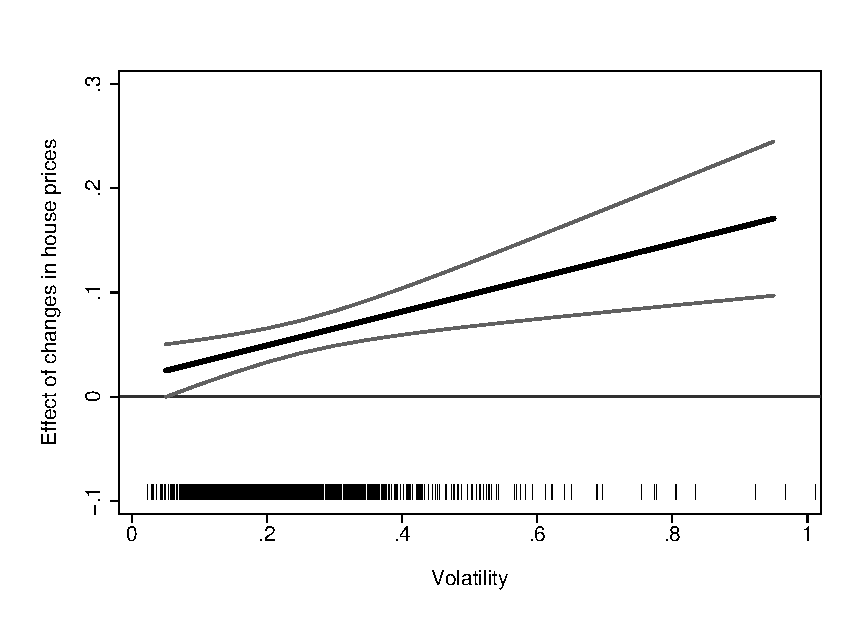
\includegraphics[width=0.8\textwidth]{../figures/volatilityinteraction.eps}
	\centering
	\caption{Marginal effect of $\Delta$house prices on incumbent support across levels of price volatility with 95 pct. Confidence Intervals. Rug plot signifies distribution of observations across the volatility variable.}
\end{figure}

\begin{table}[htbp]\centering
\def\sym#1{\ifmmode^{#1}\else\(^{#1}\)\fi}
\caption{Estimated effects of house prices on electoral support for governing parties across volatility.} \label{tab6}
\begin{tabular}{l*{5}{c}}
\hline\hline
                    &\multicolumn{1}{c}{(1)}        &\multicolumn{1}{c}{(2)}        &\multicolumn{1}{c}{(3)}        &\multicolumn{1}{c}{(4)}        &\multicolumn{1}{c}{(5)}        \\
\hline
$\Delta$ house price (positive)&        0.15\sym{**}&        0.11\sym{**}&        0.02        &        0.03        &       -0.04\sym{*} \\
                    &      (0.03)        &      (0.04)        &      (0.03)        &      (0.02)        &      (0.02)        \\
[1em]
$\Delta$ house price (negative)&       -0.05        &       -0.16\sym{*} &        0.03        &        0.02        &       -0.07\sym{*} \\
                    &      (0.07)        &      (0.06)        &      (0.05)        &      (0.05)        &      (0.03)        \\
[1em]
Volatility          &       -7.22        &        0.14        &        7.29\sym{**}&       -1.16        &       -1.73        \\
                    &      (3.72)        &      (3.25)        &      (2.70)        &      (2.03)        &      (1.60)        \\
[1em]
$\Delta$ house price (positive) $\times$ Volatility&       -0.10        &        0.04        &        0.05        &        0.03        &        0.19\sym{**}\\
                    &      (0.12)        &      (0.13)        &      (0.09)        &      (0.07)        &      (0.06)        \\
[1em]
$\Delta$ house price (negative) $\times$ Volatility&       -0.01        &        0.19        &       -0.54\sym{**}&       -0.50\sym{**}&        0.12        \\
                    &      (0.28)        &      (0.24)        &      (0.21)        &      (0.17)        &      (0.12)        \\
[1em]
\hline Precinct FE  &                    &$\checkmark$        &$\checkmark$        &$\checkmark$        &$\checkmark$        \\
[1em]
Year FE             &                    &                    &$\checkmark$        &$\checkmark$        &$\checkmark$        \\
[1em]
Year FE * Structural factors&                    &                    &                    &$\checkmark$        &$\checkmark$        \\
[1em]
Year FE * Municipality FE&                    &                    &                    &                    &$\checkmark$        \\
\hline
Observations        &        4184        &        4184        &        4184        &        4162        &        4162        \\
RMSE                &        8.46        &        7.17        &        5.70        &        4.76        &        2.84        \\
\hline\hline
\multicolumn{6}{l}{\footnotesize Standard errors in parentheses}\\
\multicolumn{6}{l}{\footnotesize \sym{*} \(p<0.05\), \sym{**} \(p<0.01\)}\\
\end{tabular}
\end{table}





\section{Discussion}

How causally convincing is our results?

Is the negativity bias really a bias? Maybe... maybe not.  ff

Implications for policy makers.

Goodnight!



%Appendikser
%Overvej et om forhold mellem volatilitet og prisændringer
%Overvej et på et andet kontekstuelt niveau - e.g. kommuner - jf. MAUP.
%Overvej et om robusthed af interaktionsled - evt. lav kommuneinteraktioner, og se om effekten stadig holder
%Overvej det samme som sidste om positiv-negativ
%Overvej om vi skal lave et datasæt med "stabile valgsteder" 
%Overvej om vi får samme resultater med statsministerpartiet.





\clearpage

\singlespacing

\bibliographystyle{apa}
\bibliography{library}

\end{document}
